\section{Concept 2 - Component/structure editor}
This section presents the second requirement-to-test translation concept, proposes a rudimentary meta model and evaluates the approach in terms which parts should be refined in a later concept, and which shouldn't.
The second concept originated from the idea that structure, could be added by component-oriented tool. The user interface only provides graphical components that represent domain actors and concepts than can be connected and re-arranged to create the use cases. The user interface should then -- similar to the first concept -- providing immediate visual feedback in the form of textual use case representation (or a diagram), like in the first concept.\\\\\
The procedure of the concept is to define actors and concepts beforehand, and then compose use cases from these. So, if starting from scratch, a user would be expected to initially define at least one actor and the actions that the actor perform, and the objects that this action would -- prior to actually writing the use case.\\\\
\begin{figure}[!htbp]
\includegraphics[scale=0.4]{\imgdir test_case_ui}
\centering
\caption{Use case editor UI mockup}
\label{fig:use_case_editor_mockup}
\end{figure}A user interface mock-up is shown in figure \ref{fig:use_case_editor_mockup}. In the top of the screen is tab selector that navigates the selected use case. In the selected use case panel, we can see the main scenario (the selected tab), where the list use case entries are shown. The selected entry is ``Receptionist send Message'', which is also shown in the bottom of the user interface where it can be edited. The available actors and concepts are shown on the right side of the user interface. The pre- and postconditions are part of the user interface, but is included in the meta model discussion.\\\\
The component/structure concept had the big advantage, that it was a good fit for -- and aided the development of -- the meta model. This concept was not chosen, due to the significantly increased workload that it involved, and the added complexity. The concept and its corresponding meta model was simplified, and was refined for the next concept.

\subsection{Meta model}
This section contains a brief discussion of a meta model that could be used for translating use cases into test cases in this concept. The discussion is supported by the high-level graphical model depicted in figure \ref{fig:concept2_use_case_meta_model}, which show the concepts that are being discussed.\\\\
\begin{figure}[h]
  \centering
  \includegraphics[scale=0.72]{\imgdir concept2_use_case_meta_model}
  \caption{Partial meta model for creating use cases models in concept 2}
  \label{fig:concept2_use_case_meta_model}
\end{figure}The central point of the meta model is the use case. It is composed of stakeholders and a primary actor, pre- and post-conditions, use case entries (the Entry class) and a number of extensions. The primary actor is mostly for information purposes, as the Actor class (which models the domain actor) is also contained within the entries. The Entry class model the use case's entries, and are not very flexible as they expect a use case entry to consist of an actor, a target and an action. The target may be either a domain actor or a domain concept.\\
The extensions are treated as lists of use case entries as well as the main scenario. In addition; they have extension points as well as optional return points to use cases. These map to the formulations where an actor returns to a specific entry in the main scenario -- for example ``user returns to 2.'' -- in extensions. The pre- and postconditions are modeled as predicate classes, that ensures that some property must hold for an associated concept.

\subsection{Mapping to application domain}
In order to map the models produced with the tool, we need to translate them to models usable by the ``test mapping domain''. Figure \ref{fig:concept2_use_case_mapping} shows the conceptual model of how a meta model supporting this domain could look like. The discussion in this section will go into too much depth with the meta model, as it has not been chosen as implementation model. There may also be inaccuracies in it, for that exact reason.
\begin{figure}[!htbp]
  \centering
  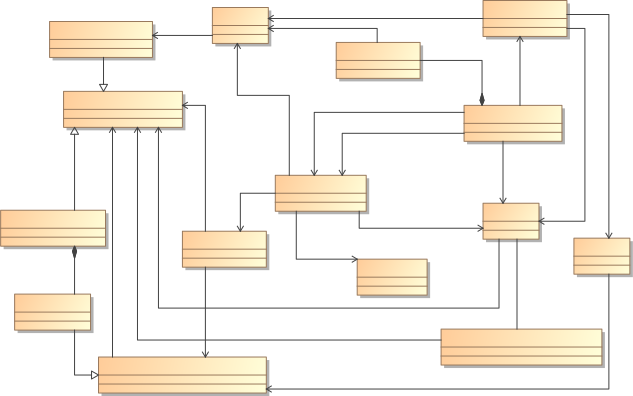
\includegraphics[scale=0.72]{img/concept2_use_case_mapping}
  \caption{Concept 2 use case mapping}
  \label{fig:concept2_use_case_mapping}
\end{figure}It specifies, like the meta model in figure \ref{fig:concept2_use_case_meta_model}, that the use case consists of an ordered list of entries, where actions consist of; one or more actors, one verb describing the action and one target for the action (object for verb). It also contains the corresponding associations to predicates (pre- and postconditions) and actors. But, unlike the simpler model for building the use case models, it is extended with additional classes, needed to construct models suitable for test generation. The mapping process is expected to be done by a developer, and could be realized by a textual test mapping language, discussed later in this section.\\\\
In the application domain, we have a set of domain actor, and domain concepts. The actors from the use case domain may be mapped to domain actors, acting in a specific role. In our system -- for example -- a ``contact'' actor may act as the ``callee'' in some use cases, which effectively is a role. A domain actor needs to specialized by application domain actor classes, that needs to be mostly coded by hand, but could be stubbed out by the tool. The wrapper class has the purpose of covering the domain concepts, functionality-wise. It will supply a set of methods, available for the developer to map to use case actions -- hence the association to the action class.\\
Predicates are treated as functional expressions, that link to a matcher which must be realized (in code) by a function that returns a boolean value, based on input. For instance, quantifications such as ``greater than'' and ``equals'' are examples of matchers.\\\\
One thing that proved useful, was the parameters of the test class. Basically, to be able to specify which domain concepts should be part of the signature of the test function. An example would be that a test function involving a receptionist actor, would need to have the signature \texttt{exampleTest(Receptionist r)}, or similar. The basic is just that the involved concepts, needs to be supplied to the test function from the test support framework.
\subsection{Mapping language}
In order to define the mappings from the requirement concept in the meta model, the concept of a mapping language emerged. While the language never left the conceptual state, it is described in this section for completeness.\\\\
The aspect of the mapping language is that of the actor. It is conceptually the same as a recipe for a holder-class (class as i object-oriented programming) that knows about every interface that it needs to access, and every resources that needs to be provided to it.\\\\
The example language shown in figure \ref{lst:mapping_language_concept} illustrates how a language like that could look like. The example uses indentions to indicate ownerships. The label ``Receptionist:'' indicates that the mappings and properties below is owned by that actor. The requirements -- which could translate to class fields -- are listed (new-line separated) below the ``requires:'' keyword. the ``maps:'' keyword translates to provided methods (as those from the figure \ref{fig:concept2_use_case_mapping}). The methods have a signature, and a function body that should translate into a class method with the supplied body.
\newpage
\begin{lstlisting}[caption=example language for mapping concepts,label={lst:mapping_language_concept}]:
Receptionist:
  requires:
    MessageContentGenerator messageContentGenerator
    ReceptionistState currentState = ReceptionistState.Unknown
  
  provides:
    changeState (ReceptionistState rs) -> currentState = rs
  
  maps:
    sends_message (Message msg) -> msg.enqueue()

    types_in (Message msg) -> 
      msg.content = messageContentGenerator.next().content
    
    returns_to (ReceptionistState newState) -> this.changeState (newState)

  properties:
    is_ready -> receptionistState == ready
\end{lstlisting}

\subsection{Evaluation}
%TODO finish this section
One of the problems with this solution is that you also need to specify who is performing the action, and who is the target.

It was too far from acutally writing the use cases. Having to decompose the use case before acutally wiritinh it is not very user friendly. 
A big problem with this approach is that it could quickly lead to artificial or too technical jargon in use cases, which is generally a bad idea as it alienates the customer \cite{christel1992}.
%TODO What are the good parts?

% What you cannot do, when having two actors, is specify the direction of the action.
The predicates provided little, or no value and could be written in the mapping code very easily without the need to include them in the meta model.

The problem with the mapping language is that is came very close to a programming class, and it felt very much like re-inventing object-oriented programming classes. The very big benefit of having a mapping language, was that the meta model of could be linked to that of our use cases, and provide a much better analysis of the use case translation. Like, which mappings were missing and such.
